\documentclass{article}

\usepackage{tikz}
\usetikzlibrary{arrows,positioning,fit,calc,shapes.geometric}

\begin{document}
\begin{figure}
  \centerline{
    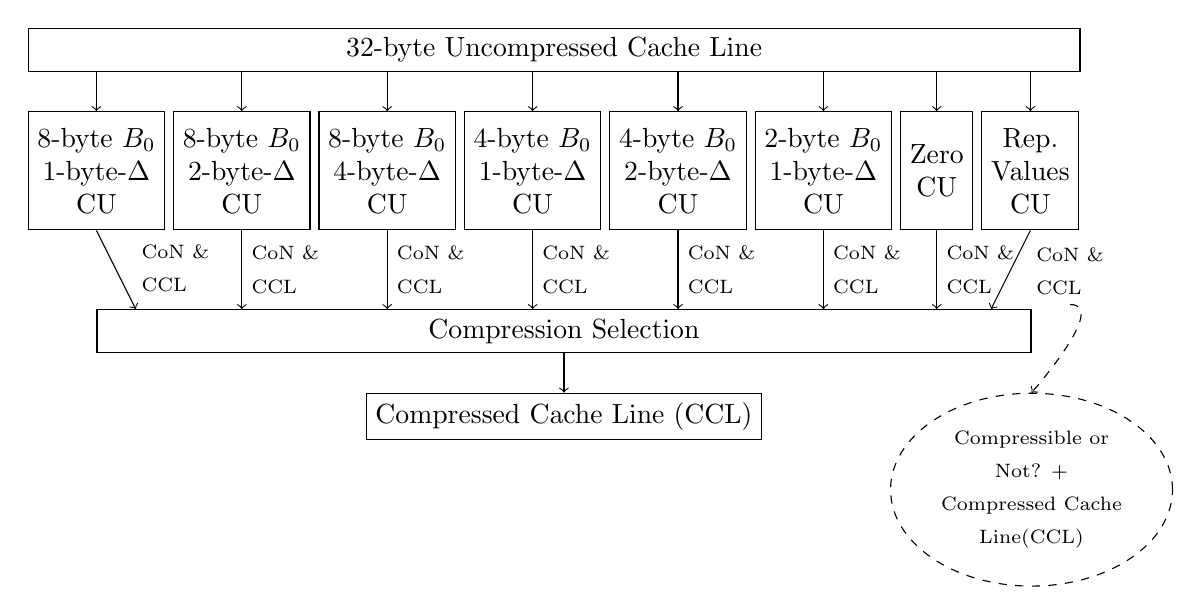
\begin{tikzpicture}[node distance=1mm]
      \node [draw,minimum height=1.5cm,align=center] (8-1-cu) {8-byte $B_0$\\ 1-byte-$\Delta$\\ CU};
      \node [draw,minimum height=1.5cm,align=center] (8-2-cu) [right=of 8-1-cu] {8-byte $B_0$\\ 2-byte-$\Delta$\\ CU};
      \node [draw,minimum height=1.5cm,align=center] (8-4-cu) [right=of 8-2-cu] {8-byte $B_0$\\ 4-byte-$\Delta$\\ CU};
      \node [draw,minimum height=1.5cm,align=center] (4-1-cu) [right=of 8-4-cu] {4-byte $B_0$\\ 1-byte-$\Delta$\\ CU};
      \node [draw,minimum height=1.5cm,align=center] (4-2-cu) [right=of 4-1-cu] {4-byte $B_0$\\ 2-byte-$\Delta$\\ CU};
      \node [draw,minimum height=1.5cm,align=center] (2-1-cu) [right=of 4-2-cu] {2-byte $B_0$\\ 1-byte-$\Delta$\\ CU};
      \node [draw,minimum height=1.5cm,align=center] (zero-cu) [right=of 2-1-cu] {Zero\\ CU};
      \node [draw,minimum height=1.5cm,align=center] (rv-cu) [right=of zero-cu] {Rep.\\ Values\\ CU};

      \path let \p1=(8-1-cu.north west), \p2=(rv-cu.north east) in (8-1-cu.west) to (rv-cu.east) node[draw,above=0.5cm of 8-1-cu.north west,minimum width=\x2-\x1,anchor=south west] (upper-line) {32-byte Uncompressed Cache Line};

      \foreach \t in {8-1-cu.north,8-2-cu.north,8-4-cu.north,4-1-cu.north,4-2-cu.north,2-1-cu.north,zero-cu.north,rv-cu.north} {
        \draw[<-] (\t) -- ++(0, 0.5);
      }

      \path let \p1=(8-1-cu.south), \p2=(rv-cu.south) in (8-1-cu) to (rv-cu) node[draw,below=1cm of 8-1-cu.south,anchor=north west,minimum width=\x2-\x1] (lower-line) {Compression Selection};

      \draw[->] (8-1-cu.south) -- ++(0.5, -1cm) node[auto,pos=.9,align=left] {\scriptsize CoN \&\\ \scriptsize CCL};
      \draw[->] (rv-cu.south) -- ++(-0.5, -1cm) node[auto,pos=.1,align=left] (last-text) {\scriptsize CoN \&\\ \scriptsize CCL};
      \foreach \t in {8-2-cu.south,8-4-cu.south,4-1-cu.south,4-2-cu.south,2-1-cu.south,zero-cu.south}{
        \draw[->] (\t) -- ++(0, -1cm) node[auto,pos=.5,align=left] {\scriptsize CoN \&\\ \scriptsize CCL};
      }

      \node[draw] (last-line) [below=0.5cm of lower-line] {Compressed Cache Line (CCL)};
      \draw[->] (lower-line.south) -- (last-line.north);

      \node[draw,dashed,ellipse,align=center] (info) [below=0.5cm of lower-line.south east,anchor=north] {\scriptsize Compressible or\\\scriptsize Not? +\\\scriptsize Compressed Cache\\\scriptsize Line(CCL)};

      \draw[dashed,->] (last-text.south) .. controls +(right:5mm) and +(up:0mm) .. (info.north);
  \end{tikzpicture}
  }
\end{figure}

\end{document}
